\section{Results}\label{sec:results}
\subsection{The Reference-Size Law on Single Trials}
Fig.~\ref{fig:law} shows cross-participant single-trial accuracy as a function of the reference size. In every paradigm accuracy rises with $m$ along the curve of Proposition~\ref{prop:law}. Over the 30 points (five paradigms, six sizes) the mean absolute difference between observed and predicted balanced accuracy is 0.004 and the largest is 0.017, at $m=1$ in N170. The prediction uses the all-trial accuracy of each paradigm, so agreement at $m=32$ is close by construction, and the informative comparison is at small $m$: for $m\ge2$ the mean absolute difference is 0.003. At $m=1$ the observed value is below the prediction in four paradigms, the direction expected from the between-class term $\Sigma_\mu/m$ of a reference drawn without regard to class.

\begin{figure*}[t]
\centering
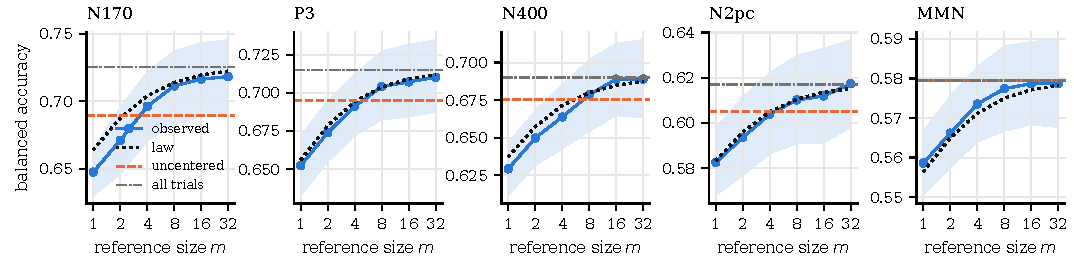
\includegraphics[width=\textwidth]{figures/fig_law.pdf}
\caption{Reference-size law on single trials of ERP CORE, cross-participant decoding, chance 0.5. Observed balanced accuracy with participant-bootstrap 95\% intervals against the prediction $\Phi(\Phi^{-1}(\BA_\infty)\sqrt{m/(m+1)})$, which uses the all-trial accuracy alone. Dashed: uncentered readout. Mean absolute error over the 30 points is 0.004.}
\label{fig:law}
\end{figure*}

Table~\ref{tab:erpcore} gives the end points. Centering on all trials of the test participant raises accuracy by 0.036 [0.021, 0.052] for N170, 0.020 for P3, 0.015 for N400, and 0.012 for N2pc, and leaves MMN unchanged ($-0.000$ [$-0.002$, $+0.002$]). The causal running mean reaches 0.721, 0.710, 0.684, 0.616, and 0.580, within 0.006 of the all-trial value in every paradigm, so the transform has an online form. Below the break-even size centering lowers accuracy: with one reference trial N170 falls from 0.690 to 0.648. Corollary~\ref{cor:breakeven} predicts the crossing from the two end points alone, at $m^\ast=2.2$, 4.2, 5.2, and 4.0, and never for MMN, where the participant share is zero. On the tested grid the first size above the uncentered readout is 4, 8, 8, and 8, and none for MMN, each the smallest grid value above its $m^\ast$. For N2pc, whose predicted break-even size is 4.0, accuracy at $m=4$ equals the uncentered value to three decimals (0.604 against 0.605).

\begin{table*}[t]
\centering
\caption{ERP CORE. Left: participant-condition averages, complete two-condition panels (chance 0.5). Right: cross-participant single-trial decoding with the participant mean taken over all trials, the gain over the uncentered readout with participant-bootstrap 95\% interval, the gain of Euclidean alignment, the break-even reference size $m^\ast$ predicted by \eqref{eq:breakeven}, and the smallest tested $m\in\{1,2,4,8,16,32\}$ whose accuracy exceeds the uncentered readout.}
\label{tab:erpcore}
\begin{tabular}{lcc|cccccc}
\toprule
 & \multicolumn{2}{c|}{Averages} & \multicolumn{6}{c}{Single trials} \\
Paradigm & Uncentered & Panel centered & Uncentered & Centered & Centering gain & Alignment gain & $m^\ast$ & First $m$ above \\
\midrule
N170 & 0.735 & 0.965 & 0.690 & 0.725 & $+0.036$ [$+0.021$, $+0.052$] & $+0.004$ [$-0.011$, $+0.020$] & 2.2 & 4 \\
P3 & 0.832 & 0.995 & 0.695 & 0.715 & $+0.020$ [$+0.007$, $+0.031$] & $-0.003$ [$-0.019$, $+0.012$] & 4.2 & 8 \\
N400 & 0.868 & 1.000 & 0.675 & 0.690 & $+0.015$ [$+0.003$, $+0.027$] & $-0.008$ [$-0.021$, $+0.005$] & 5.2 & 8 \\
N2pc & 0.636 & 0.867 & 0.605 & 0.617 & $+0.012$ [$+0.006$, $+0.018$] & $+0.010$ [$-0.001$, $+0.020$] & 4.0 & 8 \\
MMN & 0.872 & 0.955 & 0.580 & 0.579 & $-0.000$ [$-0.002$, $+0.002$] & $+0.005$ [$-0.000$, $+0.011$] & $\infty$ & none \\
\bottomrule
\end{tabular}
\end{table*}


\subsection{Complete Panels}
With participant-condition averages the participant share is large and the panel is complete. On ERP CORE, panel centering raises two-class accuracy in all five paradigms (Table~\ref{tab:erpcore}), for example from 0.735 to 0.965 for N170 and from 0.636 to 0.867 for N2pc, each above its within-participant permutation null ($p=0.002$, the floor of 500 permutations). On SHAPE, with three conditions and 211 participants, the uncentered readout scores 0.679 and full-panel centering 0.900, a gain of $+0.221$ [$+0.188$, $+0.256$], against a within-participant permutation null with mean 0.335 and maximum 0.403 over 100 permutations. Leave-one-out centering scores 0.904, as \eqref{eq:loo} requires of a rescaled copy of the same features. A panel of two of the three conditions gives 0.820, and a single observation, for which no reference exists, is decoded by the uncentered readout at 0.679. A readout trained on centered panels and applied to an uncentered single observation scores 0.509. The gain persists when the input is scaled by per-epoch z-scoring or by its pre-stimulus standard deviation ($+0.203$ and $+0.219$ on the 212-participant cohort of the original analysis), so it is not produced by per-epoch scaling. In the flattened epoch the participant factor carries 70.6\% of the variance, the condition factor 8.8\%, and the residual 20.6\%.

\begin{table}[t]
\centering
\caption{SHAPE, three affective conditions (chance 0.333), 211 participants, unscaled epochs, participant-grouped 10-fold cross-validation. Balanced accuracy with participant-bootstrap 95\% intervals. Every transform uses only the participant's own unlabeled panel.}
\label{tab:shape}
\begin{tabular}{llc}
\toprule
Transform & Order & Balanced accuracy \\
\midrule
None & -- & 0.679 [0.646, 0.712] \\
Euclidean alignment & second & 0.834 [0.806, 0.863] \\
Tangent space, cohort reference & -- & 0.472 [0.439, 0.507] \\
Tangent space, participant recentering & second & 0.727 [0.690, 0.765] \\
Panel centering & first & 0.900 [0.872, 0.927] \\
Panel centering and scaling & first & 0.905 [0.875, 0.932] \\
Euclidean alignment, then centering & both & 0.912 [0.883, 0.937] \\
Panel centering, joint assignment & first & 0.953 [0.926, 0.976] \\
\bottomrule
\end{tabular}
\end{table}


\subsection{Alignment Alternatives and Joint Assignment}
Table~\ref{tab:shape} compares transforms that use the same unlabeled panel. Euclidean alignment reaches 0.834, a gain of $+0.155$ [$+0.120$, $+0.190$] over the uncentered readout. The prediction written before the run, that a second-order transform would stay near the uncentered readout as the additive model implies, was not borne out on these averages, and it held on single trials (Table~\ref{tab:erpcore}). Centering exceeds alignment by $+0.066$ [$+0.036$, $+0.096$], and alignment followed by centering scores 0.912, a difference of $+0.011$ [$-0.017$, $+0.038$] from centering alone. Adding a per-feature scale from the three-observation panel changes centering by $+0.005$ [$-0.016$, $+0.027$]. In the covariance domain, tangent-space features with a cohort reference score 0.472 and participant recentering raises them to 0.727 ($+0.253$ [$+0.209$, $+0.299$]). These features discard the time course of the average, which accounts for their lower level. Joint assignment of the three labels of each test panel raises the centered readout from 0.900 to 0.953, a gain of $+0.052$ [$+0.028$, $+0.076$] that comes entirely from the known composition of the panel.
